\documentclass[9pt]{developercv}
\begin{document}
\begin{minipage}[t]{0.45\textwidth}
	\vspace{-\baselineskip}
	\colorbox{black}{{\HUGE\textcolor{white}{\textbf{\MakeUppercase{Samuel}}}}}
	\colorbox{black}{{\HUGE\textcolor{white}{\textbf{\MakeUppercase{Kyletoft}}}}}
	\vspace{6pt}
\end{minipage}
\begin{minipage}[t]{0.275\textwidth}
	\vspace{-\baselineskip}
	\icon{MapMarker}{12}{Gothenburg, Sweden}\\
	\icon{Phone}{12}{+46 761 76 53 67}\\
	\icon{At}{12}{\href{mailto:samuel@kyletoft.se}{samuel@kyletoft.se}}\\	
\end{minipage}
\begin{minipage}[t]{0.275\textwidth}
	\vspace{-\baselineskip}
	\icon{Globe}{12}{\href{https://samuel.kyletoft.se}{samuel.kyletoft.se}}\\
	\icon{Github}{12}{\href{https://github.com/SKyletoft}{/SKyletoft}}\\
	\icon{Linkedin}{12}{\href{https://www.linkedin.com/in/samuel-kyletoft}{/samuel-kyletoft}}\\
\end{minipage}\\

\vspace{0.5cm}

\begin{minipage}[t]{0.7\textwidth}
	\vspace{-\baselineskip}
	\cvsect{Who am I?}
	\\Born in 2000 in Stockholm, Sweden och currently a student studying Computer
	Science and Engineering at Chalmers University of Technology in Gothenburg.
	\\ With an interest in compilers and performance.
\end{minipage}
\hfill
\begin{minipage}[t]{0.2\textwidth}
	\vspace{-\baselineskip}
	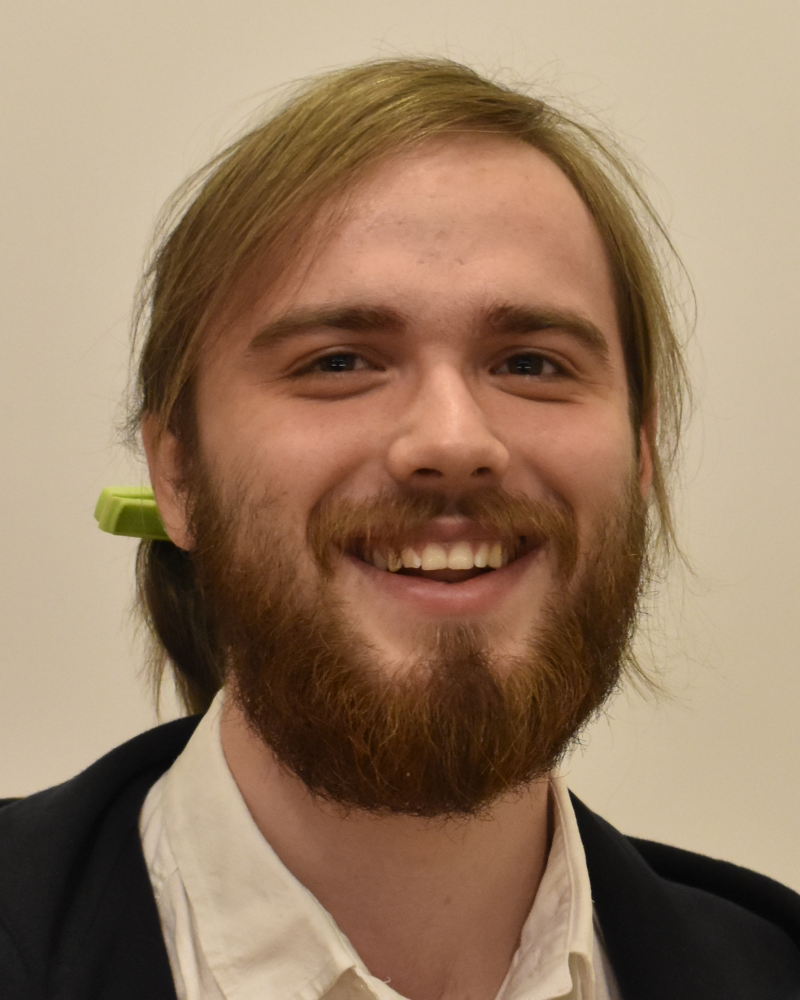
\includegraphics[width=\linewidth]{smaller.png}
\end{minipage}
\cvsect{Education}
\begin{entrylist}
	\entry
		{2020 -- }
		{(Ongoing, Yr 3) Computer Science and Engineering (MSc) (300 Credits)}
		{Chalmers Univeristy of Technology}
		{Civilingenjör Datateknik}
	\entry
		{Spring 2020}
		{Basic Course in Law (15 Credits)}
		{Uppsala Univeristy}
		{Juridisk Översiktskurs}
	\entry
		{2016 -- 2019}
		{Natural Sciences Programme}
		{Norra Real's Gymnasium (High School)}
		{Naturvetenskapsprogrammet}
\end{entrylist}
\cvsect{Experience}
\begin{entrylist}
	\entry
		{August 2021 -- }
		{Teaching Assistant/Amanuens}
		{Chalmers University of Technology}
		{
			As a TA I've run labs, helped students in their classes and
			graded labs and exams.\\ I have TA'd the following classes:\\
			\texttt{Introduction to Functional Programming}\slashsep
			\texttt{Introduction to Computer Engineering}\slashsep
			\texttt{Machine Oriented Programmering}\slashsep
			\texttt{Introduction to Object Oriented Programming}\slashsep
			\texttt{Principles of Concurrent Programming}
		}
	\entry
		{May 2022 \\-- May 2023}
		{Board member}
		{Career and Business Relations Committee at the CSE Student Division (DAG)}
		{
			As a board member of DAG I have worked with
			businesses to sponsor the student division through
			lunch lectures, pub nights and trips to visit
			companies.\\
		}
	\entry
		{May 2021 \\-- May 2022}
		{Server Maintainer}
		{Server Committee at the CSE Student Division (dHack)}
		{
			During my year in dHack I ran the divisions servers and services and started new ones.\\
		}
\end{entrylist}
\begin{minipage}[t]{0.3\textwidth}
	\vspace{-\baselineskip}
	\cvsect{Languages}\\
	\textbf{Swedish} - fluent\\
	\textbf{English} - fluent
\end{minipage}
\hfill
\begin{minipage}[t]{0.3\textwidth}
	\vspace{-\baselineskip}
	\cvsect{Hobbies}
	\\During weekends I often take long walks through the woods and work
	on implementing a compiler for the custom Artemis programming language.
	\\ Before I moved to Gothenburg I was active in my local scout corps and
	orienteering club.
\end{minipage}
\hfill
\begin{minipage}[t]{0.3\textwidth}
	\vspace{-\baselineskip}
	\cvsect{Other skills}
	\\I have a Swedish standard driver's license.
\end{minipage}
\end{document}
